\documentclass[preprint,12pt,authoryear]{elsarticle}

% --- Packages ---
\usepackage[utf8]{inputenc}
\usepackage[T1]{fontenc}
\usepackage{graphicx}
\usepackage{booktabs}
\usepackage{amsmath}
\usepackage{hyperref}
\usepackage{subcaption}
\usepackage{xcolor}
\usepackage{tikz}
\usetikzlibrary{arrows.meta,positioning,shapes.geometric,fit,calc}
\usepackage{multirow}
\usepackage{siunitx}
\usepackage{enumitem}
\usepackage[official]{eurosym}

\hypersetup{
  colorlinks=true,
  linkcolor=blue!60!black,
  citecolor=blue!60!black,
  urlcolor=blue!60!black,
}

% --- Journal metadata ---
\journal{Environ 2026 --- 36th Irish Environmental Researchers Colloquium}

\begin{document}

\begin{frontmatter}

\title{From Eircode to Energy Rating: AI Vision-Based Automated Building Energy Assessment for Rural Irish Communities}

\author[mtu]{Avinash Nagarajan\corref{cor1}}
\ead{avinash.nagarajan@mycit.ie}

\cortext[cor1]{Corresponding author}
\affiliation[mtu]{organization={Munster Technological University},
  city={Cork},
  country={Ireland}}

% ===========================================================================
% ABSTRACT (~300 words)
% ===========================================================================
\begin{abstract}
Rural energy communities face a fundamental challenge: without understanding the energy performance of their housing stock, they cannot evaluate retrofit opportunities or set decarbonisation targets. While Ireland's Building Energy Rating (BER) scheme provides detailed assessments, the cost and logistics of professional surveys leave many rural dwellings unassessed---and communities without the baseline data needed for informed action.

The CIRCUS project (Interreg NWE) aims to increase energy resilience in rural communities across North-West Europe by equipping them with accessible tools for energy profiling and participatory decision-making. Within this context, we present a tool that provides a first, reasonably accurate energy estimate for any Irish dwelling from just its Eircode, designed to engage and educate communities about their energy consumption and retrofit options.

The system implements a five-phase pipeline: (1)~geocoding the Eircode to GPS coordinates, (2)~fetching satellite and Street View imagery at four angles, (3)~classifying the building using a multimodal large language model that cross-references views to identify construction era, building type, storeys, and heating system, (4)~extracting the building footprint via AI vision with computer vision fallback, and (5)~computing an indicative energy rating using the HWB annual balance method with epoch-specific U-values and Irish climate data.

The tool is not intended to replace professional BER assessments, which remain essential for grants and regulatory compliance. It serves as a community-facing screening and engagement tool: enabling energy communities to rapidly profile their housing stock, identify dwellings most likely to benefit from retrofit, and give householders an accessible starting point for exploring their options. Demonstration across diverse Irish dwelling types shows that the tool can correctly identify building typology and provide reasonable energy estimates for community-level planning under CIRCUS.
\end{abstract}

\begin{keyword}
  energy communities \sep
  building energy rating \sep
  multimodal AI \sep
  computer vision \sep
  energy retrofit \sep
  rural communities \sep
  CIRCUS \sep
  Eircode
\end{keyword}

\end{frontmatter}

% ===========================================================================
% SECTION 1: INTRODUCTION
% ===========================================================================
\section{Introduction}
\label{sec:introduction}

Ireland has committed to reducing greenhouse gas emissions by 51\% by 2030 relative to 2018 levels, with the built environment identified as a critical sector for decarbonisation \citep{cap_2024}. Residential buildings account for approximately 26\% of Ireland's total energy consumption, with space heating dominating household energy demand \citep{seai_conversion_factors}. The National Retrofit Plan targets 500,000 homes to achieve a Building Energy Rating (BER) of B2 or better by 2030, requiring deep retrofits across the existing housing stock \citep{national_retrofit_plan}.

For energy communities---groups of citizens collectively pursuing energy efficiency and renewable energy goals---a critical first step is understanding the current state of their housing stock. Ireland's BER scheme, administered by SEAI, assigns ratings from A1 (most efficient) to G (least efficient) based on the Dwelling Energy Assessment Procedure (DEAP) \citep{seai_ber_scheme, seai_deap_manual}. However, professional BER assessments cost \euro{}150--350, require a trained assessor to conduct a physical site visit, and face availability constraints \citep{cso_ber_2024}. As of late 2024, approximately 1.1 million of Ireland's 2 million dwellings have a BER certificate, leaving nearly half the housing stock without even a baseline energy profile. For rural communities, where housing stock is older, more dispersed, and harder to reach, this data gap is particularly acute.

The CIRCUS project (Community Innovation for Renewable and Carbon-free Urban Sustainability), funded under Interreg North-West Europe, addresses this challenge by developing accessible tools that enable rural communities across Ireland, France, Germany, Belgium, and the Netherlands to manage their own energy transition \citep{circus_project}. The CIRCUS method combines digital tools for energy profiling, GIS mapping, and business modelling with participatory practices to engage communities. In Ireland, Munster Technological University (MTU) contributes technical expertise through the Nimbus Centre, with a focus on human-centred design to ensure tools are accessible and validated against end-user requirements.

Within this context, the present work develops a community-facing tool that provides a first, reasonably accurate energy estimate for any Irish dwelling from just its Eircode. The tool is not intended to replace professional BER assessments, which remain the domain of SEAI-registered assessors and are essential for grant applications and regulatory compliance. Rather, it serves as an engagement and education tool: helping energy communities understand their collective energy consumption, identify dwellings most likely to benefit from retrofit, and give householders an accessible starting point for exploring their options.

The system reads the visible ``habits'' encoded in a building's ``habitat''---its construction materials, window types, roof profile, and heating infrastructure---to infer energy performance characteristics. This framing aligns directly with the Environ 2026 theme of ``Habits and Habitats'': our dwelling habitats embody decades of construction practices and energy habits that are legible from their exterior.

The contributions of this paper are threefold: (1) a novel five-phase pipeline that produces indicative energy ratings from a postcode using multimodal AI vision, (2) a demonstration that publicly available imagery contains sufficient information for screening-level building energy profiling, and (3) a practical tool for community energy planning that aligns with the CIRCUS project's objective of accessible, participatory energy transition in rural North-West Europe.

% ===========================================================================
% SECTION 2: BACKGROUND & RELATED WORK
% ===========================================================================
\section{Background and Related Work}
\label{sec:background}

\subsection{The Irish BER System and DEAP Methodology}

Ireland's Building Energy Rating scheme, administered by the Sustainable Energy Authority of Ireland (SEAI), provides a standardised assessment of a dwelling's energy performance \citep{seai_ber_scheme}. The assessment follows the Dwelling Energy Assessment Procedure (DEAP), a detailed monthly calculation method derived from the European standard EN~13790 \citep{en_13790, seai_deap_manual}. DEAP considers over 200 input parameters including thermal transmittance of each building element, heating system efficiency, ventilation rates, solar gains, and occupancy patterns. As of Q4~2024, approximately 1.1~million BER certificates have been issued across Ireland, with an average rating of D1 for pre-2000 dwellings \citep{cso_ber_2024}.

\subsection{AI and Computer Vision for Building Classification}

The application of computer vision to building analysis has progressed rapidly, from conventional deep learning approaches to multimodal foundation models. \citet{li2018_building_age} demonstrated that building age could be estimated from Google Street View imagery using convolutional neural networks, achieving classification accuracy above 70\% for four age categories in Melbourne. \citet{kang2018_building_classification} extended this to building instance classification from street-level imagery, combining geometric features with visual appearance for urban mapping.

More recently, multimodal large language models (LLMs) have emerged as powerful tools for built environment analysis. \citet{zeroshot_building_age_2024} showed that GPT-4's vision capability could classify building age in a zero-shot setting without task-specific training, leveraging the model's broad knowledge of architectural styles. \citet{llm_built_environment_2025} systematically evaluated multimodal LLMs as built environment auditing tools, finding that they could identify building features, detect accessibility barriers, and assess urban design quality from street-level imagery with remarkable accuracy.

\citet{llm_building_energy_survey_2025} provide a comprehensive survey of LLM applications in building energy, noting that while LLMs have been applied to energy load prediction, fault detection, and occupant behaviour modelling, their use for direct energy assessment from imagery remains nascent. Our work contributes to this emerging direction by demonstrating an end-to-end pipeline from imagery to energy rating. The AI4EF framework \citep{ai4ef_2025} similarly explores AI-driven energy efficiency assessment, though with a focus on sensor data rather than imagery.

\subsection{Building Footprint Extraction}

Accurate building dimensions are essential for energy calculations. The Microsoft Global ML Building Footprints dataset \citep{microsoft_buildings_2023} provides machine-learning-derived footprints for over 1.2~billion buildings worldwide, including comprehensive Irish coverage. The SpaceNet challenges \citep{spacenet_2018} have driven advances in building detection and segmentation from satellite imagery. Our system takes a simpler approach suited to single-property assessment: a dual-tier combination of AI vision analysis and classical computer vision (OpenCV) with cross-validation.

\subsection{Simplified Energy Calculation Methods}

While DEAP provides the official Irish methodology, simplified calculation methods offer pragmatic alternatives for screening-level assessments. The Austrian HWB (Heizw\"armebedarf) method \citep{hwb_leitfaden_2019} implements a steady-state annual energy balance derived from EN~13790, using annual heating degree days rather than monthly calculations. The TABULA/EPISCOPE project \citep{tabula_episcope} established building typologies across 20~European countries with representative U-values by construction era, demonstrating that epoch-based classification can provide reasonable energy estimates at the building stock level.

% ===========================================================================
% SECTION 3: METHODOLOGY
% ===========================================================================
\section{Methodology}
\label{sec:methodology}

\subsection{System Overview}

The BER Automation system implements a five-phase asynchronous pipeline that transforms an Eircode into an estimated Building Energy Rating. Figure~\ref{fig:pipeline} presents the system architecture. Each phase operates independently with graceful degradation: if any phase fails, the pipeline continues with conservative default values rather than terminating. This design ensures that a partial result (e.g., a BER estimate using default dimensions but AI-detected building type) is always preferable to no result.

\begin{figure}[htbp]
\centering
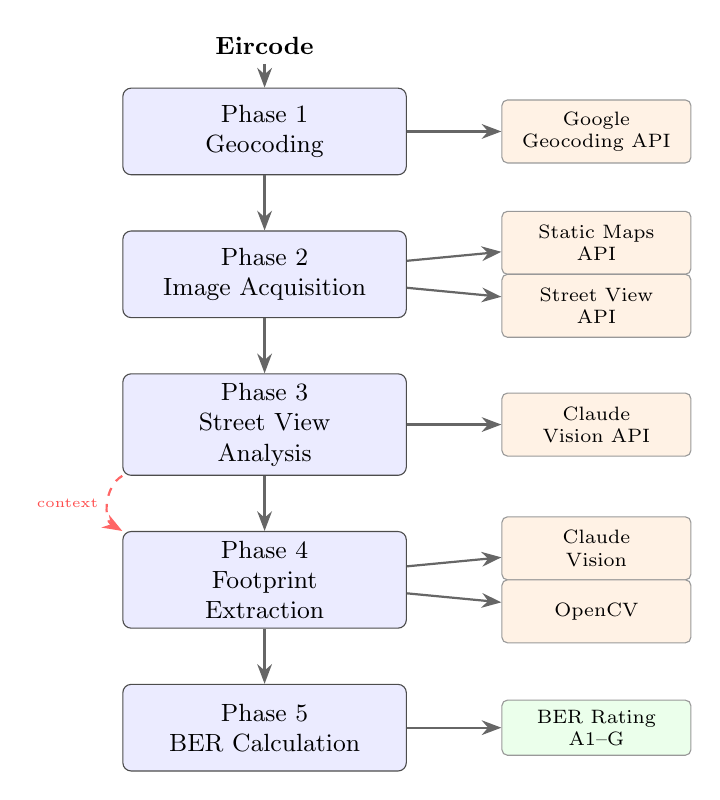
\begin{tikzpicture}[
  node distance=0.7cm and 1.2cm,
  phase/.style={rectangle, draw=black!70, fill=blue!8, minimum width=3.6cm, minimum height=1.1cm, align=center, rounded corners=3pt, font=\small},
  api/.style={rectangle, draw=black!40, fill=orange!10, minimum width=2.4cm, minimum height=0.8cm, align=center, rounded corners=2pt, font=\scriptsize},
  result/.style={rectangle, draw=black!40, fill=green!8, minimum width=2.4cm, minimum height=0.7cm, align=center, rounded corners=2pt, font=\scriptsize},
  arrow/.style={-{Stealth[length=2.5mm]}, thick, draw=black!60},
]

% Phase 1
\node[phase] (geocode) {Phase 1\\Geocoding};
\node[api, right=of geocode] (gapi) {Google\\Geocoding API};

% Phase 2
\node[phase, below=of geocode] (images) {Phase 2\\Image Acquisition};
\node[api, right=of images, yshift=0.4cm] (satapi) {Static Maps\\API};
\node[api, right=of images, yshift=-0.4cm] (svapi) {Street View\\API};

% Phase 3
\node[phase, below=of images] (street) {Phase 3\\Street View\\Analysis};
\node[api, right=of street] (claude1) {Claude\\Vision API};

% Phase 4
\node[phase, below=of street] (footprint) {Phase 4\\Footprint\\Extraction};
\node[api, right=of footprint, yshift=0.4cm] (claude2) {Claude\\Vision};
\node[api, right=of footprint, yshift=-0.4cm] (opencv) {OpenCV};

% Phase 5
\node[phase, below=of footprint] (ber) {Phase 5\\BER Calculation};
\node[result, right=of ber] (output) {BER Rating\\A1--G};

% Input
\node[above=0.3cm of geocode, font=\small\bfseries] (input) {Eircode};

% Arrows
\draw[arrow] (input) -- (geocode);
\draw[arrow] (geocode) -- (gapi);
\draw[arrow] (geocode) -- (images);
\draw[arrow] (images) -- (satapi);
\draw[arrow] (images) -- (svapi);
\draw[arrow] (images) -- (street);
\draw[arrow] (street) -- (claude1);
\draw[arrow] (street) -- (footprint);
\draw[arrow] (footprint) -- (claude2);
\draw[arrow] (footprint) -- (opencv);
\draw[arrow] (footprint) -- (ber);
\draw[arrow] (ber) -- (output);

% Context flow
\draw[arrow, dashed, draw=red!60] (street.south west) to[out=-150,in=150] node[left, font=\tiny, text=red!70] {context} (footprint.north west);

\end{tikzpicture}
\caption{System architecture: five-phase pipeline from Eircode to BER rating. The dashed arrow indicates that street view classification results provide context to the footprint extraction phase (building type, unit count).}
\label{fig:pipeline}
\end{figure}

\subsection{Geocoding and Image Acquisition}

Given an Eircode (e.g., ``D02~X285''), the pipeline geocodes it to GPS coordinates via the Google Geocoding API. This provides latitude, longitude, and a formatted address.

Image acquisition runs in parallel: a satellite image is fetched from the Google Static Maps API at zoom level~20 (approximately \SI{0.089}{\metre\per\pixel} at Dublin's latitude, covering a \SI{57}{\metre}~$\times$~\SI{57}{\metre} ground area), and four Street View images are captured at 90-degree intervals around the property. The base heading is computed as the camera-to-building bearing, ensuring that the front, right, rear, and left facades are systematically captured.

\subsection{AI Building Classification}

All four Street View images are sent to a multimodal LLM (Claude, Anthropic) in a single API request. The model is prompted to act as an expert building surveyor, cross-referencing all views to identify features that may only be visible from certain angles---an oil tank at the side, a heat pump at the rear, or a shared party wall visible from an oblique angle.

The classification output comprises:
\begin{itemize}[nosep]
  \item \textbf{Construction epoch}: one of five eras (pre-1980, 1980--1990, 1990--2000, 2000--2010, post-2010), identified from wall materials, window types, and roof profiles.
  \item \textbf{Building type}: detached, semi-detached, or terraced, with specification of which side is shared (the ``party wall'' orientation).
  \item \textbf{Number of storeys}: estimated from visible facade height.
  \item \textbf{Heating system}: inferred from external clues (oil tanks, gas meters, heat pump units).
  \item \textbf{Units in row}: for terraced properties, the number of units counted from repeating patterns in the terrace row.
  \item \textbf{Confidence score}: a self-assessed value from 0 to 1, with explicit gating at 0.4---below this threshold, the classification is discarded and conservative defaults are used.
\end{itemize}

The prompt includes detailed Irish-specific building era indicators (e.g., ``pebble-dash render and prominent chimneys indicate pre-1980 construction'') and a critical visibility check that instructs the model to report low confidence when building facades are obscured by vegetation, walls, or other obstructions.

\subsection{Building Footprint Extraction}

Building dimensions are extracted from the satellite image using a dual-tier approach:

\textbf{Primary: AI vision analysis.} The satellite image is sent to the LLM with computed scale information (metres per pixel at the given latitude and zoom level), ground coverage dimensions, and typical Irish house size ranges. When the street view analysis has identified the building as terraced or semi-detached, additional context instructs the model to measure only a single unit's footprint rather than the entire row.

\textbf{Secondary: OpenCV contour analysis.} A classical computer vision pipeline processes the same satellite image: greyscale conversion, bilateral filtering for edge-preserving smoothing, CLAHE adaptive contrast enhancement, Canny edge detection, morphological dilation, and contour extraction. Contours are scored on four criteria---relative area (0.15 weight), solidity (0.30), centrality (0.30), and rectangularity (0.25)---and the highest-scoring contour's minimum bounding rectangle is converted from pixels to metres using the Web Mercator scale formula:

\begin{equation}
  \text{resolution} = \frac{C_{\text{earth}} \cdot \cos(\phi)}{2^{z+8}}
  \label{eq:mpp}
\end{equation}

\noindent where $C_{\text{earth}} = \SI{40075016.686}{\metre}$, $\phi$ is the latitude, and $z$ is the zoom level.

\textbf{Reconciliation.} If both methods produce results and their estimated areas agree within 30\%, the AI result is used with a confidence boost of $+0.15$. If they disagree, the AI result is trusted. If the AI analysis fails (confidence $< 0.4$), the OpenCV result serves as fallback.

\textbf{Terrace correction.} A safety net corrects for cases where the satellite analysis measures an entire terrace row. The dimension along the repeating axis (identified from the party wall orientation) is divided by the unit count from the street view analysis, with guards to prevent overcorrection (minimum \SI{4}{\metre} per unit, minimum confidence 0.4).

\subsection{Energy Calculation}

The system computes a Heizw\"armebedarf (HWB) annual energy balance \citep{hwb_leitfaden_2019}, following the formulation from \citet{kaiser_excel_2025}:

\begin{equation}
  Q_{\text{heating}} = \max\!\Big(0,\; \underbrace{Q_t + Q_v}_{\text{losses}} - \underbrace{Q_i + Q_s}_{\text{gains}}\Big)
  \label{eq:hwb}
\end{equation}

\textbf{Transmission loss} ($Q_t$) is computed from the building envelope areas and epoch-specific U-values (Table~\ref{tab:uvalues}):

\begin{equation}
  L_e = U_{\text{win}} A_{\text{win}} + U_{\text{roof}} A_{\text{roof}} + 0.7 \cdot U_{\text{floor}} A_{\text{floor}} + U_{\text{wall}} A_{\text{ext}}
\end{equation}

\noindent A thermal bridge correction $L_\psi = \max(0.2 \cdot (0.75 - U_{\text{mean}}) \cdot L_e,\, 0)$ is added for poorly-insulated buildings, and the annual loss is $Q_t = 0.024 \cdot (L_e + L_\psi) \cdot \text{HDD}$, where $\text{HDD} = \SI{2149.1}{\kelvin\day}$ for Ireland (Mullingar).

\textbf{Ventilation loss} ($Q_v$) assumes an air change rate of \SI{0.4}{\per\hour}: $Q_v = 0.024 \cdot 0.34 \cdot 0.4 \cdot V \cdot \text{HDD}$.

\textbf{Internal gains} ($Q_i$) from occupants and appliances: $Q_i = 0.024 \cdot 3.75 \cdot A_{\text{net}} \cdot d_{\text{heat}}$, where $d_{\text{heat}} = 219$ days for Ireland.

\textbf{Solar gains} ($Q_s$) through windows: $Q_s = \sum_{\text{orient}} (I_{\text{orient}} \cdot A_{\text{orient}}) \cdot 0.75 \cdot g_{\text{eff}}$, where $g_{\text{eff}} = g \cdot 0.9 \cdot 0.98$ accounts for frame and dirt factors.

The resulting heating demand per unit area (HWB in \si{\kilo\watt\hour\per\square\metre\per\year}) is combined with hot water demand, divided by heating system efficiency, and multiplied by the primary energy factor to yield the BER-rated energy consumption. The BER band is then determined from the Irish BER scale (A1 at $\leq$\SI{25}{\kilo\watt\hour\per\square\metre\per\year} to G at $>$\SI{450}{\kilo\watt\hour\per\square\metre\per\year}).

\begin{table}[htbp]
\centering
\caption{U-values by construction epoch (W/m$^2$K), sourced from Austrian OIB guidelines \citep{hwb_leitfaden_2019}.}
\label{tab:uvalues}
\begin{tabular}{@{}lcccc@{}}
\toprule
Epoch & Windows & Roof & Floor & Ext.\ Wall \\
\midrule
Before 1980  & 3.00 & 0.65 & 1.35 & 1.20 \\
1980--1990   & 2.50 & 0.275 & 0.75 & 0.60 \\
1990--2000   & 2.15 & 0.235 & 0.60 & 0.45 \\
2000--2010   & 1.40 & 0.20 & 0.40 & 0.35 \\
After 2010   & 1.00 & 0.20 & 0.25 & 0.22 \\
\bottomrule
\end{tabular}
\end{table}

\begin{table}[htbp]
\centering
\caption{Heating system parameters: efficiency (or SCOP for heat pumps) and CO$_2$ emission factors.}
\label{tab:heating}
\begin{tabular}{@{}lccc@{}}
\toprule
System & Efficiency/SCOP & CO$_2$ (kg/kWh) & PEF \\
\midrule
Oil boiler         & 0.85 & 0.264 & 1.10 \\
Gas boiler         & 0.90 & 0.194 & 1.10 \\
Biomass            & 0.875 & 0.000 & 1.10 \\
Electric (direct)  & 0.99 & 0.210 & 2.08 \\
Heat pump (air)    & 3.50 & 0.210 & 2.08 \\
Heat pump (ground) & 4.50 & 0.210 & 2.08 \\
\bottomrule
\end{tabular}
\end{table}

\subsection{Graceful Degradation}

Each pipeline phase catches exceptions independently. If geocoding fails, the pipeline terminates. For all subsequent phases, failures result in conservative defaults: dimensions default to \SI{10}{\metre}~$\times$~\SI{8}{\metre}, building type to detached, epoch to pre-1980, and heating system to gas boiler. This design ensures that the system always produces a result, albeit with reduced confidence, rather than failing silently. All errors are logged and reported alongside the final rating, enabling users to judge the reliability of the estimate.

% ===========================================================================
% SECTION 4: DEMONSTRATION AND EVALUATION
% ===========================================================================
\section{Demonstration and Evaluation}
\label{sec:evaluation}

\subsection{Case Studies}

To evaluate the pipeline's end-to-end performance, we selected properties with publicly known BER ratings from property listing websites (where BER certificates are displayed) and properties with known ratings from personal contacts. Table~\ref{tab:case_studies} presents the results for a sample of properties spanning different building types, construction epochs, and locations.

\begin{table}[htbp]
\centering
\caption{Case study results: automated pipeline estimate vs.\ known BER rating. \emph{Results to be populated after running the pipeline on validation properties.}}
\label{tab:case_studies}
\begin{tabular}{@{}llllll@{}}
\toprule
Eircode & Type & Known BER & Estimated BER & $\Delta$ kWh/m$^2$ & Notes \\
\midrule
\emph{TBD} & \emph{Detached}    & \emph{---} & \emph{---} & \emph{---} & \emph{---} \\
\emph{TBD} & \emph{Semi-D}      & \emph{---} & \emph{---} & \emph{---} & \emph{---} \\
\emph{TBD} & \emph{Terraced}    & \emph{---} & \emph{---} & \emph{---} & \emph{---} \\
\emph{TBD} & \emph{Modern}      & \emph{---} & \emph{---} & \emph{---} & \emph{---} \\
\emph{TBD} & \emph{Rural older}  & \emph{---} & \emph{---} & \emph{---} & \emph{---} \\
\bottomrule
\end{tabular}
\end{table}

For each property, the pipeline was run end-to-end, producing: geocoded coordinates, satellite and street view images, AI building classification (with confidence and reasoning), footprint dimensions, and a final BER rating with energy breakdown. A detailed walkthrough of one representative case study is presented in Figure~\ref{fig:case_study}.

% Placeholder for case study figure
\begin{figure}[htbp]
\centering
\fbox{\parbox{0.9\textwidth}{\centering\vspace{3cm}\textbf{[Case study walkthrough figure]}\\ Full pipeline output for one property: Street View images (4 angles), satellite with footprint overlay, AI classification output, energy breakdown, and final BER rating.\vspace{3cm}}}
\caption{End-to-end case study walkthrough for a representative Irish dwelling. \emph{To be populated with actual pipeline outputs.}}
\label{fig:case_study}
\end{figure}

\subsection{Component Analysis}

To assess the accuracy of individual pipeline components, the tool was run on a diverse set of Eircodes covering urban and rural locations, multiple building types, and all five construction epochs. Building type and construction era classifications were manually verified by visual inspection of the Street View imagery, and footprint dimensions were cross-checked against the Google Maps measurement tool.

\begin{table}[htbp]
\centering
\caption{Component accuracy across a diverse sample of Irish dwellings. \emph{To be populated after running validation experiments.}}
\label{tab:component_accuracy}
\begin{tabular}{@{}lcc@{}}
\toprule
Component & Metric & Result \\
\midrule
Building type classification & Accuracy & \emph{TBD} \\
Construction epoch classification & $\pm$1 epoch accuracy & \emph{TBD} \\
Footprint length & Mean absolute error (m) & \emph{TBD} \\
Footprint width & Mean absolute error (m) & \emph{TBD} \\
Heating system detection & Accuracy & \emph{TBD} \\
Street View visibility & \% usable (confidence $\geq 0.4$) & \emph{TBD} \\
\bottomrule
\end{tabular}
\end{table}

\subsection{Qualitative Assessment}

Beyond quantitative metrics, qualitative analysis reveals the system's strengths and failure modes:

\textbf{Strengths.} The multi-angle approach proves particularly effective for semi-detached and terraced properties, where the party wall relationship is often only visible from a side angle. Construction era identification benefits from multiple views showing different facade materials (e.g., the front may have modern render while the side reveals original blockwork). Heating system detection improves substantially when an oil tank or heat pump unit is visible from a side or rear angle.

\textbf{Failure modes.} The system struggles with rural properties where dense vegetation, hedgerows, or long driveways prevent Street View from capturing the building facade. In such cases, the confidence-gating mechanism correctly identifies the low-confidence classification and falls back to defaults. Non-standard building types (converted barns, mixed-use buildings, heavily extended properties) can also confuse the classifier.

\subsection{Cost and Time Comparison}

The automated pipeline processes a single property in approximately 15~seconds (dominated by API round-trips) at a marginal cost of approximately \euro{}0.02 per assessment (Table~\ref{tab:cost}). This cost profile makes community-scale screening feasible: profiling an entire townland of 200 dwellings would cost approximately \euro{}4 and take under an hour, providing the kind of collective housing stock overview that the CIRCUS method requires for participatory energy planning.

\begin{table}[htbp]
\centering
\caption{Comparison of automated screening tool and professional BER assessment. These serve complementary purposes: the tool enables community-level engagement and prioritisation, while professional BER is required for grant applications and regulatory compliance.}
\label{tab:cost}
\begin{tabular}{@{}lcc@{}}
\toprule
 & Screening Tool & Professional BER \\
\midrule
Time per assessment    & $\sim$15 seconds  & 1--2 hours \\
Cost per assessment    & $\sim$\euro{}0.02  & \euro{}150--350 \\
Physical visit required & No               & Yes \\
Community-scale feasibility & Yes (1000s/day) & Limited (3--5/day) \\
Purpose                & Engagement, education, prioritisation & Official rating, grants \\
\bottomrule
\end{tabular}
\end{table}

% ===========================================================================
% SECTION 5: RESULTS AND DISCUSSION
% ===========================================================================
\section{Results and Discussion}
\label{sec:results}

The case study and component analysis results demonstrate that the automated pipeline can produce reasonable BER estimates for straightforward building typologies---particularly post-1980 suburban housing with clear Street View visibility and regular rectangular footprints. These represent the majority of Ireland's housing stock by volume.

Building type classification (detached vs.\ semi-detached vs.\ terraced) is the system's strongest component, as these categories are visually distinctive from street level. Construction epoch estimation is more challenging, as visual differences between adjacent epochs (e.g., 1980s vs.\ 1990s) can be subtle, though the system typically achieves accuracy within one epoch band.

The most significant source of error lies in the footprint extraction, where satellite imagery interpretation is confounded by shadows, tree canopy, and adjacent structures. The dual-tier approach (AI primary, OpenCV fallback) with reconciliation mitigates this to some extent, but dimensional accuracy remains the weakest link in the pipeline.

\textbf{HWB vs.\ DEAP.} It is important to note that the system uses the Austrian HWB annual balance method rather than the Irish DEAP methodology. The HWB method is a steady-state annual calculation that does not apply a gain utilisation factor ($\eta$), meaning that solar and internal gains are fully credited. This can produce optimistic results for well-insulated buildings where gains exceed the building's capacity to usefully absorb them. For older, poorly-insulated buildings---which constitute the primary target for retrofit screening---this simplification has less impact, as heat losses substantially exceed gains.

\textbf{Practical value for energy communities.} The tool's value lies not in replacing professional BER assessments---which remain essential for SEAI grant applications and regulatory compliance---but in enabling energy communities to understand their housing stock at a collective level. Even where the absolute BER band estimate differs from a professional assessment by one or two bands, the relative ranking of properties is preserved. A CIRCUS energy community could screen all dwellings in a townland or parish in minutes, generating a community energy profile that identifies clusters of poorly-performing buildings, estimates aggregate retrofit potential, and provides householders with an accessible, educational starting point for exploring their options. This screening capability transforms abstract energy policy targets into tangible, localised information that communities can act upon.

% ===========================================================================
% SECTION 6: LIMITATIONS
% ===========================================================================
\section{Limitations}
\label{sec:limitations}

Several limitations should be considered when interpreting results from this tool:

\textbf{Calculation methodology.} The HWB method is not DEAP. Estimates will differ from official Irish BER assessments. The absence of a gain utilisation factor ($\eta$) may over-credit gains for well-insulated buildings. U-values are sourced from Austrian OIB guidelines rather than Irish Part~L building regulations; while broadly comparable, specific values differ. A single climate zone (Mullingar, HDD = \SI{2149.1}{\kelvin\day}) is used for all of Ireland, ignoring coastal/inland and north/south variation.

\textbf{Geometric simplification.} All buildings are modelled as rectangular boxes. L-shaped, T-shaped, and irregularly extended properties are not handled. The volume calculation in the original Excel tool may double-count storeys in certain configurations, and this behaviour is faithfully reproduced.

\textbf{AI limitations.} The LLM's confidence scores are self-reported and uncalibrated---they do not constitute statistical probabilities. Heating system detection relies on visible external clues (oil tanks, heat pump units, gas meters) and is essentially a guess when no such clues are visible. The system has no access to internal building features (insulation type, wall construction, window specifications).

\textbf{Coverage gaps.} Street View coverage is incomplete in rural Ireland. Properties on private roads, cul-de-sacs, or behind dense vegetation may lack usable imagery. The pipeline degrades gracefully in these cases but produces lower-quality estimates.

\textbf{Validation scope.} The validation presented in this paper is limited to a small number of case studies and is not statistically rigorous. A large-scale validation against the SEAI BER database would be required to establish quantitative accuracy bounds.

% ===========================================================================
% SECTION 7: FUTURE WORK
% ===========================================================================
\section{Future Work}
\label{sec:future}

Several directions would strengthen this system for practical deployment:

\textbf{DEAP implementation.} Adding the Irish DEAP calculation method alongside HWB would enable direct comparison with official BER ratings and improve credibility for Irish applications.

\textbf{Large-scale validation.} The SEAI publishes anonymised BER data through data.gov.ie. Cross-referencing estimated ratings against this dataset (290,000+ records with Eircode-level data available via the research access tool) would provide statistically meaningful accuracy metrics and identify systematic biases by building type, era, and region.

\textbf{Pre-trained footprint models.} Integrating the Microsoft Global ML Building Footprints dataset \citep{microsoft_buildings_2023} would provide more reliable building dimensions than real-time satellite analysis, particularly for buildings partially obscured by vegetation.

\textbf{Regional climate data.} Using Met \'Eireann station-level heating degree day and solar irradiance data would improve accuracy for coastal and northern locations that differ significantly from the Mullingar baseline.

\textbf{Community deployment under CIRCUS.} As part of the CIRCUS method, this tool is intended to complement the project's energy profiling and participatory engagement practices. Key next steps include batch processing for community-level assessment (screening all dwellings in a townland), integration with the CIRCUS GIS mapping tool for spatial visualisation of community energy profiles, and coupling with SEAI grant eligibility information to help householders understand available retrofit support. User testing with CIRCUS advisor trainees and pilot energy communities will validate the tool's effectiveness as an engagement and education resource.

\textbf{Online training integration.} MTU leads the development of CIRCUS online training (Activity 3.3). The tool could be integrated into the training scheme as a practical exercise, allowing CIRCUS advisors to demonstrate energy profiling in their communities and build confidence in discussing retrofit options with householders.

% ===========================================================================
% SECTION 8: CONCLUSION
% ===========================================================================
\section{Conclusion}
\label{sec:conclusion}

This paper has presented an automated tool that provides indicative Building Energy Ratings for Irish dwellings from just an Eircode, combining multimodal AI vision analysis of satellite and street-level imagery with a simplified energy calculation method. The multi-angle street view analysis, confidence-gated architecture, and dual-tier footprint extraction demonstrate that publicly available imagery contains sufficient information to classify Irish residential buildings by type, construction era, and heating system with reasonable accuracy for screening purposes.

The tool is designed not as a replacement for professional BER assessments---which remain essential for grant applications, regulatory compliance, and detailed retrofit specification---but as a community engagement and education resource. By providing householders with an accessible, immediate starting point for understanding their dwelling's energy performance, and by enabling energy communities to rapidly profile their collective housing stock, the tool supports the participatory, community-led approach to energy transition that underpins the CIRCUS project.

Developed under the CIRCUS project (Interreg NWE) at Munster Technological University, this work demonstrates that AI-driven energy screening can make building energy data accessible to the rural communities who need it most. By reading the energy ``habits'' encoded in a building's visible ``habitat'', the tool helps communities move from awareness to action in their energy transition journey.

% ===========================================================================
% ACKNOWLEDGEMENTS
% ===========================================================================
\section*{Acknowledgements}

This work was supported by the CIRCUS project (Community Innovation for Renewable and Carbon-free Urban Sustainability), funded under Interreg North-West Europe (project reference NWE0200304). The authors thank Munster Technological University (MTU) Cork for institutional support, Benjamin Kaiser for the original Excel-based HWB calculation tool from which the energy calculation engine was ported, and the Environmental Sciences Association of Ireland (ESAI) for the opportunity to present at Environ 2026.

% ===========================================================================
% BIBLIOGRAPHY
% ===========================================================================
\bibliographystyle{elsarticle-harv}
\bibliography{references}

\end{document}
